\documentclass[aspectratio=169]{beamer}
\usepackage[utf8]{inputenc}
\usepackage[T1]{fontenc}
\usepackage[brazil]{babel}
\usepackage{ragged2e}
\usepackage{booktabs}
\usepackage{verbatim}
\usetheme{AnnArbor}
\usecolortheme{orchid}
\usefonttheme[onlymath]{serif}
%\usepackage{listings}
\usepackage{listingsutf8}
\usepackage{colortbl}
\usepackage{array}

\newcolumntype{C}[0]{>{\centering\arraybackslash}p{0.4cm}}

\lstset{language=C++,
	inputencoding=utf8/latin1,	
	backgroundcolor=\color{green!10},
	basicstyle=\ttfamily,
	keywordstyle=\color{blue}\ttfamily,
	stringstyle=\color{red}\ttfamily,
	commentstyle=\color{green}\ttfamily,
	morecomment=[l][\color{magenta}]{\#}
}

\AtBeginSection[]{
  \begin{frame}
  \vfill
  \centering
  \begin{beamercolorbox}[sep=8pt,center,shadow=true,rounded=true]{title}
    \usebeamerfont{title}\insertsectionhead\par%
  \end{beamercolorbox}
  \vfill
  \end{frame}
}

\title[\sc{Algoritmos de Ordenação}]{Algoritmos de Ordenação}
\author[Roland Teodorowitsch]{Roland Teodorowitsch}
\institute[ALEST I - EP - PUCRS]{Algoritmos e Estruturas de Dados I - Escola Politécnica - PUCRS}
\date{8 de outubror de 2023}

\begin{document}

\justifying

%-------------------------------------------------------
\begin{frame}
	\titlepage
\end{frame}

%=======================================================
\section{Introdução}

%-------------------------------------------------------
\begin{frame}\frametitle{Leitura(s) Recomendada(s)}

\begin{columns}[T]
\begin{column}{0.15\linewidth}
\vspace{-3mm}
\begin{figure}[h]
	\centering
	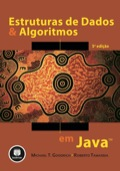
\includegraphics[height=0.3\paperheight]{imagens/livro_goodrich.jpg}
\end{figure}
\end{column}
\begin{column}{0.85\linewidth}
\vspace{3mm}
\textbf{Seções 3.1.2, 11.1 (\emph{Merge Sort}), 11.2 (\emph{Quick Sort}), 11.3.3 (comparação)}\\
\scriptsize{GOODRICH, Michael T.; TAMASSIA, Roberto. \textbf{Estruturas de dados e algoritmos em Java}. Tradução: Bernardo Copstein. 5. ed. Porto Alegre: Bookman, 2013. xxii, 713 p. E-book. ISBN 9788582600191. Tradução de: Data Structures and Algorithms in Java, 5th Edition. Disponível em: \textless{}\url{https://integrada.minhabiblioteca.com.br/\#/books/9788582600191/}\textgreater{}. Acesso em: 01 ago. 2023.}
\end{column}
\end{columns}

\end{frame}

%-------------------------------------------------------
\begin{frame}\frametitle{Sites sobre Ordenação [*]}
\begin{itemize}
{\small
	\item Animações:\\\url{http://www.sorting-algorithms.com/}
	\item Algoritmos na wikipedia:\\\url {https://en.wikipedia.org/wiki/Sorting_algorithm}
	\item Danças:\\\url{http://makezine.com/2011/04/12/data-sorting-dances/}
	\item 15 algoritmos em 6 minutos:\\\url{https://www.youtube.com/watch?v=kPRA0W1kECg}
	\item Visualização e comparação de algoritmos de ordenação:\\\url{https://www.youtube.com/watch?v=ZZuD6iUe3Pc}
	\item Visualização \emph{Bubble Sort vs Quick Sort}:\\\url{https://www.youtube.com/watch?v=aXXWXz5rF64}
	\item Visualização \emph{Merge Sort vs Quick Sort}:\\\url{https://www.youtube.com/watch?v=es2T6KY45cA}
}
\end{itemize}
\end{frame}

%-------------------------------------------------------
\begin{frame}\frametitle{Revisão: Algoritmos de Pesquisa}
\begin{itemize}
	\item Pesquisa Linear
	\begin{itemize}
		\item Pode ser aplicada sobre qualquer coleção, ordenada ou não
		\item Procura um item, comparando-o com cada elemento da coleção, até achar ou chegar no final
		\item Melhor caso: o item procurado está na primeira posição da coleção
		\item Pior caso: o item NÃO está na coleção
		\item Complexidade: $O(n)$
	\end{itemize}
	\item Pesquisa Binária
	\begin{itemize}
		\item A coleção deve estar ordenada
		\item Estratégia básica:
		\begin{itemize}
			\item Verifica o elemento central: se encontrou, a busca termina
			\item Se o item for menor que o central, considera apenas a parte abaixo do elemento central
			\item Se o item for maior que o central, considera apenas a parte acima do elemento central
		\end{itemize}
		\item Trabalha subdividindo a coleção e reaplicando sempre a estratégia básica, o que o torna adequado para implementação recursiva
		\item Complexidade: $O(\log n)$
	\end{itemize}
\end{itemize}
\end{frame}

%=======================================================
\section{Algoritmos de Ordenação}

%-------------------------------------------------------
\begin{frame}\frametitle{Algoritmos de Ordenação}
\begin{itemize}
	\item Organizam os elementos de uma coleção segundo determinado critério (ordem crescente de valor, por exemplo)
	\item Operação básica: troca de elementos
	\item Exemplos
	\begin{itemize}
		\item \emph{Bubble Sort}
		\item \emph{Selection Sort}
		\item \emph{Insertion Sort}
		\item \emph{Merge Sort}
		\item \emph{Quick Sort}
		\item etc.
	\end{itemize}
	\item Em geral, os mais simples nem sempre tem bom desempenho (menos otimizados)
	\item Algoritmos com bom desempenho costumam ser mais sofisticados
	\item São importantes quando se quer implementar busca eficiente (pesquisa binária)
\end{itemize}
\end{frame}

%=======================================================
\section{\emph{Bubble Sort}}

%-------------------------------------------------------
\begin{frame}\frametitle{\emph{Bubble Sort}}
\begin{itemize}
	\item É um dos métodos mais simples de ordenação
	\item Estratégia: compara elementos adjacentes, e, se estiverem fora de ordem, troca os elementos
	\item Repete-se a estratégia básica até que a coleção esteja ordenada
	\item Complexidade: $O(n)$ (melhor caso) ou $O(n^2)$ (pior caso)
\end{itemize}
\end{frame}

%-------------------------------------------------------
\begin{frame}\frametitle{\emph{Bubble Sort}: Exemplo}
\begin{center}
\begin{tabular}{CCCCCCCCCC}
\tiny{0} & \tiny{1} & \tiny{2} & \tiny{3} & \tiny{4} & \tiny{5} & \tiny{6} & \tiny{7} & \tiny{8} & \tiny{9}\\
\hline
\multicolumn{1}{|C|}{5} & \multicolumn{1}{|C|}{7} & \multicolumn{1}{|C|}{8} & \multicolumn{1}{|C|}{1} & \multicolumn{1}{|C|}{10} & \multicolumn{1}{|C|}{9} & \multicolumn{1}{|C|}{4} & \multicolumn{1}{|C|}{6} & \multicolumn{1}{|C|}{3} & \multicolumn{1}{|C|}{2}\\
\hline
\hline
\multicolumn{1}{|C|}{5} & \multicolumn{1}{|C|}{7} & \multicolumn{1}{|C|}{1} & \multicolumn{1}{|C|}{8} & \multicolumn{1}{|C|}{9} & \multicolumn{1}{|C|}{4} & \multicolumn{1}{|C|}{6} & \multicolumn{1}{|C|}{3} & \multicolumn{1}{|C|}{2} & \multicolumn{1}{|C|}{\cellcolor{green}10}\\
\hline
\hline
\multicolumn{1}{|C|}{5} & \multicolumn{1}{|C|}{1} & \multicolumn{1}{|C|}{7} & \multicolumn{1}{|C|}{8} & \multicolumn{1}{|C|}{4} & \multicolumn{1}{|C|}{6} & \multicolumn{1}{|C|}{3} & \multicolumn{1}{|C|}{2} & \multicolumn{1}{|C|}{\cellcolor{green}9} & \multicolumn{1}{|C|}{\cellcolor{green}10}\\
\hline
\hline
\multicolumn{1}{|C|}{1} & \multicolumn{1}{|C|}{5} & \multicolumn{1}{|C|}{7} & \multicolumn{1}{|C|}{4} & \multicolumn{1}{|C|}{6} & \multicolumn{1}{|C|}{3} & \multicolumn{1}{|C|}{2} & \multicolumn{1}{|C|}{\cellcolor{green}8} & \multicolumn{1}{|C|}{\cellcolor{green}9} & \multicolumn{1}{|C|}{\cellcolor{green}10}\\
\hline
\hline
\multicolumn{1}{|C|}{1} & \multicolumn{1}{|C|}{5} & \multicolumn{1}{|C|}{4} & \multicolumn{1}{|C|}{6} & \multicolumn{1}{|C|}{3} & \multicolumn{1}{|C|}{2} & \multicolumn{1}{|C|}{\cellcolor{green}7} & \multicolumn{1}{|C|}{\cellcolor{green}8} & \multicolumn{1}{|C|}{\cellcolor{green}9} & \multicolumn{1}{|C|}{\cellcolor{green}10}\\
\hline
\hline
\multicolumn{1}{|C|}{1} & \multicolumn{1}{|C|}{4} & \multicolumn{1}{|C|}{5} & \multicolumn{1}{|C|}{3} & \multicolumn{1}{|C|}{2} & \multicolumn{1}{|C|}{\cellcolor{green}6} & \multicolumn{1}{|C|}{\cellcolor{green}7} & \multicolumn{1}{|C|}{\cellcolor{green}8} & \multicolumn{1}{|C|}{\cellcolor{green}9} & \multicolumn{1}{|C|}{\cellcolor{green}10}\\
\hline
\hline
\multicolumn{1}{|C|}{1} & \multicolumn{1}{|C|}{4} & \multicolumn{1}{|C|}{3} & \multicolumn{1}{|C|}{2} & \multicolumn{1}{|C|}{\cellcolor{green}5} & \multicolumn{1}{|C|}{\cellcolor{green}6} & \multicolumn{1}{|C|}{\cellcolor{green}7} & \multicolumn{1}{|C|}{\cellcolor{green}8} & \multicolumn{1}{|C|}{\cellcolor{green}9} & \multicolumn{1}{|C|}{\cellcolor{green}10}\\
\hline
\hline
\multicolumn{1}{|C|}{1} & \multicolumn{1}{|C|}{3} & \multicolumn{1}{|C|}{2} & \multicolumn{1}{|C|}{\cellcolor{green}4} & \multicolumn{1}{|C|}{\cellcolor{green}5} & \multicolumn{1}{|C|}{\cellcolor{green}6} & \multicolumn{1}{|C|}{\cellcolor{green}7} & \multicolumn{1}{|C|}{\cellcolor{green}8} & \multicolumn{1}{|C|}{\cellcolor{green}9} & \multicolumn{1}{|C|}{\cellcolor{green}10}\\
\hline
\hline
\multicolumn{1}{|C|}{1} & \multicolumn{1}{|C|}{2} & \multicolumn{1}{|C|}{\cellcolor{green}3} & \multicolumn{1}{|C|}{\cellcolor{green}4} & \multicolumn{1}{|C|}{\cellcolor{green}5} & \multicolumn{1}{|C|}{\cellcolor{green}6} & \multicolumn{1}{|C|}{\cellcolor{green}7} & \multicolumn{1}{|C|}{\cellcolor{green}8} & \multicolumn{1}{|C|}{\cellcolor{green}9} & \multicolumn{1}{|C|}{\cellcolor{green}10}\\
\hline
\hline
\multicolumn{1}{|C|}{\cellcolor{green}1} & \multicolumn{1}{|C|}{\cellcolor{green}2} & \multicolumn{1}{|C|}{\cellcolor{green}3} & \multicolumn{1}{|C|}{\cellcolor{green}4} & \multicolumn{1}{|C|}{\cellcolor{green}5} & \multicolumn{1}{|C|}{\cellcolor{green}6} & \multicolumn{1}{|C|}{\cellcolor{green}7} & \multicolumn{1}{|C|}{\cellcolor{green}8} & \multicolumn{1}{|C|}{\cellcolor{green}9} & \multicolumn{1}{|C|}{\cellcolor{green}10}\\
\hline
\end{tabular}
\end{center}
\end{frame}	

%-------------------------------------------------------
\begin{frame}[fragile]\frametitle{\emph{Bubble Sort}: Implementação}
\lstinputlisting[basicstyle=\ttfamily\small]{src/bubbleSort.cpp}
\end{frame}

%-------------------------------------------------------
\begin{frame}[fragile]\frametitle{\emph{Bubble Sort}: Mais informações [*]}
\begin{itemize}
	\item \url{http://www.sorting-algorithms.com/bubble-sort}
	\item \url{https://www.hackerearth.com/practice/algorithms/sorting/bubble-sort/tutorial/}
\end{itemize}
\end{frame}

%=======================================================
\section{\emph{Selection Sort}}

%-------------------------------------------------------
\begin{frame}\frametitle{\emph{Selection Sort}}
\begin{itemize}
	\item É um algorimo de ordenação por seleção
	\item Fácil de implementar e bastante intuitivo, o que não garante eficiência...
	\item Estratégia: procurar o menor elemento e colocá-lo na sua posiçao
	\item Repete-se a estratégia até que todos os elementos estejam em sua posição
	\item Complexidade: $O(n^2)$ (melhor e pior caso)
\end{itemize}
\end{frame}

%-------------------------------------------------------
\begin{frame}\frametitle{\emph{Selection Sort}: Exemplo}
\begin{center}
\begin{tabular}{CCCCCCCCCC}
\tiny{0} & \tiny{1} & \tiny{2} & \tiny{3} & \tiny{4} & \tiny{5} & \tiny{6} & \tiny{7} & \tiny{8} & \tiny{9}\\
\hline
\multicolumn{1}{|C|}{5} & \multicolumn{1}{|C|}{7} & \multicolumn{1}{|C|}{8} & \multicolumn{1}{|C|}{1} & \multicolumn{1}{|C|}{10} & \multicolumn{1}{|C|}{9} & \multicolumn{1}{|C|}{4} & \multicolumn{1}{|C|}{6} & \multicolumn{1}{|C|}{3} & \multicolumn{1}{|C|}{2}\\
\hline
\hline
\multicolumn{1}{|C|}{\cellcolor{green}1} & \multicolumn{1}{|C|}{7} & \multicolumn{1}{|C|}{8} & \multicolumn{1}{|C|}{5} & \multicolumn{1}{|C|}{10} & \multicolumn{1}{|C|}{9} & \multicolumn{1}{|C|}{4} & \multicolumn{1}{|C|}{6} & \multicolumn{1}{|C|}{3} & \multicolumn{1}{|C|}{2}\\
\hline
\hline
\multicolumn{1}{|C|}{\cellcolor{green}1} & \multicolumn{1}{|C|}{\cellcolor{green}2} & \multicolumn{1}{|C|}{8} & \multicolumn{1}{|C|}{5} & \multicolumn{1}{|C|}{10} & \multicolumn{1}{|C|}{9} & \multicolumn{1}{|C|}{4} & \multicolumn{1}{|C|}{6} & \multicolumn{1}{|C|}{3} & \multicolumn{1}{|C|}{7}\\
\hline
\hline
\multicolumn{1}{|C|}{\cellcolor{green}1} & \multicolumn{1}{|C|}{\cellcolor{green}2} & \multicolumn{1}{|C|}{\cellcolor{green}3} & \multicolumn{1}{|C|}{5} & \multicolumn{1}{|C|}{10} & \multicolumn{1}{|C|}{9} & \multicolumn{1}{|C|}{4} & \multicolumn{1}{|C|}{6} & \multicolumn{1}{|C|}{8} & \multicolumn{1}{|C|}{7}\\
\hline
\hline
\multicolumn{1}{|C|}{\cellcolor{green}1} & \multicolumn{1}{|C|}{\cellcolor{green}2} & \multicolumn{1}{|C|}{\cellcolor{green}3} & \multicolumn{1}{|C|}{\cellcolor{green}4} & \multicolumn{1}{|C|}{10} & \multicolumn{1}{|C|}{9} & \multicolumn{1}{|C|}{5} & \multicolumn{1}{|C|}{6} & \multicolumn{1}{|C|}{8} & \multicolumn{1}{|C|}{7}\\
\hline
\hline
\multicolumn{1}{|C|}{\cellcolor{green}1} & \multicolumn{1}{|C|}{\cellcolor{green}2} & \multicolumn{1}{|C|}{\cellcolor{green}3} & \multicolumn{1}{|C|}{\cellcolor{green}4} & \multicolumn{1}{|C|}{\cellcolor{green}5} & \multicolumn{1}{|C|}{9} & \multicolumn{1}{|C|}{10} & \multicolumn{1}{|C|}{6} & \multicolumn{1}{|C|}{8} & \multicolumn{1}{|C|}{7}\\
\hline
\hline
\multicolumn{1}{|C|}{\cellcolor{green}1} & \multicolumn{1}{|C|}{\cellcolor{green}2} & \multicolumn{1}{|C|}{\cellcolor{green}3} & \multicolumn{1}{|C|}{\cellcolor{green}4} & \multicolumn{1}{|C|}{\cellcolor{green}5} & \multicolumn{1}{|C|}{\cellcolor{green}6} & \multicolumn{1}{|C|}{10} & \multicolumn{1}{|C|}{9} & \multicolumn{1}{|C|}{8} & \multicolumn{1}{|C|}{7}\\
\hline
\hline
\multicolumn{1}{|C|}{\cellcolor{green}1} & \multicolumn{1}{|C|}{\cellcolor{green}2} & \multicolumn{1}{|C|}{\cellcolor{green}3} & \multicolumn{1}{|C|}{\cellcolor{green}4} & \multicolumn{1}{|C|}{\cellcolor{green}5} & \multicolumn{1}{|C|}{\cellcolor{green}6} & \multicolumn{1}{|C|}{\cellcolor{green}7} & \multicolumn{1}{|C|}{9} & \multicolumn{1}{|C|}{8} & \multicolumn{1}{|C|}{10}\\
\hline
\hline
\multicolumn{1}{|C|}{\cellcolor{green}1} & \multicolumn{1}{|C|}{\cellcolor{green}2} & \multicolumn{1}{|C|}{\cellcolor{green}3} & \multicolumn{1}{|C|}{\cellcolor{green}4} & \multicolumn{1}{|C|}{\cellcolor{green}5} & \multicolumn{1}{|C|}{\cellcolor{green}6} & \multicolumn{1}{|C|}{\cellcolor{green}7} & \multicolumn{1}{|C|}{\cellcolor{green}8} & \multicolumn{1}{|C|}{9} & \multicolumn{1}{|C|}{10}\\
\hline
\hline
\multicolumn{1}{|C|}{\cellcolor{green}1} & \multicolumn{1}{|C|}{\cellcolor{green}2} & \multicolumn{1}{|C|}{\cellcolor{green}3} & \multicolumn{1}{|C|}{\cellcolor{green}4} & \multicolumn{1}{|C|}{\cellcolor{green}5} & \multicolumn{1}{|C|}{\cellcolor{green}6} & \multicolumn{1}{|C|}{\cellcolor{green}7} & \multicolumn{1}{|C|}{\cellcolor{green}8} & \multicolumn{1}{|C|}{\cellcolor{green}9} & \multicolumn{1}{|C|}{\cellcolor{green}10}\\
\hline
\end{tabular}
\end{center}
\end{frame}

%-------------------------------------------------------
\begin{frame}\frametitle{\emph{Selection Sort}: Implementação}
\lstinputlisting[basicstyle=\ttfamily\small]{src/selectionSort.cpp}
\end{frame}

%=======================================================
\section{\emph{Insertion Sort}}

%-------------------------------------------------------
\begin{frame}\frametitle{\emph{Insertion Sort}}
\begin{itemize}
	\item É um algorimo de ordenação por inserção
	\item Estratégia:
	\begin{itemize}
		\item Escolhe-se uma base que inicia no segundo elemento e avança até o último elemento
		\item Sempre à esquerda da base todos os elementos devem estar ordenados
		\item Busca-se a posição da base nos elementos à esquerda, sempre deslocando os elementos uma posição para a direita enquanto não chegar na posição correta da base
		\item Quando chegar na posição correta da base, atribui-se o valor da base para esta posição
	\end{itemize}
	\item Trata-se de uma algoritmo um pouco mais avançado do que os dois anteriores
	\item Complexidade: $O(n)$ (melhor caso) ou $O(n^2)$ (pior caso)
\end{itemize}
\end{frame}	

%-------------------------------------------------------
\begin{frame}\frametitle{\emph{Insertion Sort}: Exemplo 1}
\begin{figure}[h]
	\centering
	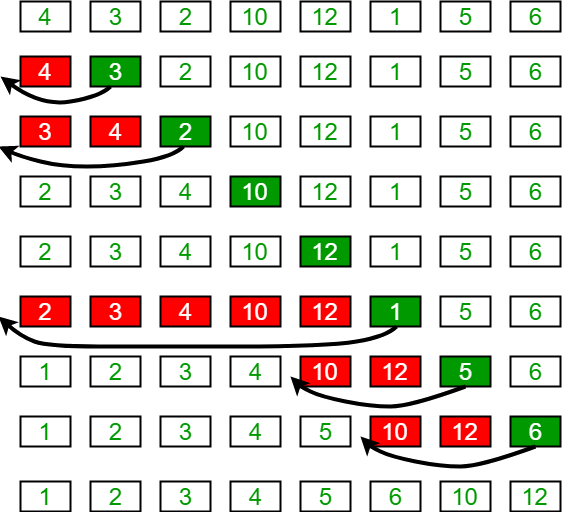
\includegraphics[height=0.6\paperheight]{imagens/insertion_sort.png}\\
	~ {\tiny Fonte: \url{https://www.geeksforgeeks.org/insertion-sort/}}
\end{figure}
\end{frame}

%-------------------------------------------------------
\begin{frame}\frametitle{\emph{Insertion Sort}: Exemplo 2}
\begin{center}
\begin{tabular}{CCCCCCCCCC}
\tiny{0} & \tiny{1} & \tiny{2} & \tiny{3} & \tiny{4} & \tiny{5} & \tiny{6} & \tiny{7} & \tiny{8} & \tiny{9}\\
\hline
\multicolumn{1}{|C|}{\cellcolor{lime}5} & \multicolumn{1}{|C|}{\cellcolor{yellow}7} & \multicolumn{1}{|C|}{8} & \multicolumn{1}{|C|}{1} & \multicolumn{1}{|C|}{10} & \multicolumn{1}{|C|}{9} & \multicolumn{1}{|C|}{4} & \multicolumn{1}{|C|}{6} & \multicolumn{1}{|C|}{3} & \multicolumn{1}{|C|}{2}\\
\hline
\hline
\multicolumn{1}{|C|}{\cellcolor{lime}5} & \multicolumn{1}{|C|}{\cellcolor{lime}7} & \multicolumn{1}{|C|}{\cellcolor{yellow}8} & \multicolumn{1}{|C|}{1} & \multicolumn{1}{|C|}{10} & \multicolumn{1}{|C|}{9} & \multicolumn{1}{|C|}{4} & \multicolumn{1}{|C|}{6} & \multicolumn{1}{|C|}{3} & \multicolumn{1}{|C|}{2}\\
\hline
\hline
\multicolumn{1}{|C|}{\cellcolor{lime}5} & \multicolumn{1}{|C|}{\cellcolor{lime}7} & \multicolumn{1}{|C|}{\cellcolor{lime}8} & \multicolumn{1}{|C|}{\cellcolor{yellow}1} & \multicolumn{1}{|C|}{10} & \multicolumn{1}{|C|}{9} & \multicolumn{1}{|C|}{4} & \multicolumn{1}{|C|}{6} & \multicolumn{1}{|C|}{3} & \multicolumn{1}{|C|}{2}\\
\hline
\hline
\multicolumn{1}{|C|}{\cellcolor{lime}1} & \multicolumn{1}{|C|}{\cellcolor{lime}5} & \multicolumn{1}{|C|}{\cellcolor{lime}7} & \multicolumn{1}{|C|}{\cellcolor{lime}8} & \multicolumn{1}{|C|}{\cellcolor{yellow}10} & \multicolumn{1}{|C|}{9} & \multicolumn{1}{|C|}{4} & \multicolumn{1}{|C|}{6} & \multicolumn{1}{|C|}{3} & \multicolumn{1}{|C|}{2}\\
\hline
\hline
\multicolumn{1}{|C|}{\cellcolor{lime}1} & \multicolumn{1}{|C|}{\cellcolor{lime}5} & \multicolumn{1}{|C|}{\cellcolor{lime}7} & \multicolumn{1}{|C|}{\cellcolor{lime}8} & \multicolumn{1}{|C|}{\cellcolor{lime}10} & \multicolumn{1}{|C|}{\cellcolor{yellow}9} & \multicolumn{1}{|C|}{4} & \multicolumn{1}{|C|}{6} & \multicolumn{1}{|C|}{3} & \multicolumn{1}{|C|}{2}\\
\hline
\hline
\multicolumn{1}{|C|}{\cellcolor{lime}1} & \multicolumn{1}{|C|}{\cellcolor{lime}5} & \multicolumn{1}{|C|}{\cellcolor{lime}7} & \multicolumn{1}{|C|}{\cellcolor{lime}8} & \multicolumn{1}{|C|}{\cellcolor{lime}9} & \multicolumn{1}{|C|}{\cellcolor{lime}10} & \multicolumn{1}{|C|}{\cellcolor{yellow}4} & \multicolumn{1}{|C|}{6} & \multicolumn{1}{|C|}{3} & \multicolumn{1}{|C|}{2}\\
\hline
\hline
\multicolumn{1}{|C|}{\cellcolor{lime}1} & \multicolumn{1}{|C|}{\cellcolor{lime}4} & \multicolumn{1}{|C|}{\cellcolor{lime}5} & \multicolumn{1}{|C|}{\cellcolor{lime}7} & \multicolumn{1}{|C|}{\cellcolor{lime}8} & \multicolumn{1}{|C|}{\cellcolor{lime}9} & \multicolumn{1}{|C|}{\cellcolor{lime}10} & \multicolumn{1}{|C|}{\cellcolor{yellow}6} & \multicolumn{1}{|C|}{3} & \multicolumn{1}{|C|}{2}\\
\hline
\hline
\multicolumn{1}{|C|}{\cellcolor{lime}1} & \multicolumn{1}{|C|}{\cellcolor{lime}4} & \multicolumn{1}{|C|}{\cellcolor{lime}5} & \multicolumn{1}{|C|}{\cellcolor{lime}6} & \multicolumn{1}{|C|}{\cellcolor{lime}7} & \multicolumn{1}{|C|}{\cellcolor{lime}8} & \multicolumn{1}{|C|}{\cellcolor{lime}9} & \multicolumn{1}{|C|}{\cellcolor{lime}10} & \multicolumn{1}{|C|}{\cellcolor{yellow}3} & \multicolumn{1}{|C|}{2}\\
\hline
\hline
\multicolumn{1}{|C|}{\cellcolor{lime}1} & \multicolumn{1}{|C|}{\cellcolor{lime}3} & \multicolumn{1}{|C|}{\cellcolor{lime}4} & \multicolumn{1}{|C|}{\cellcolor{lime}5} & \multicolumn{1}{|C|}{\cellcolor{lime}6} & \multicolumn{1}{|C|}{\cellcolor{lime}7} & \multicolumn{1}{|C|}{\cellcolor{lime}8} & \multicolumn{1}{|C|}{\cellcolor{lime}9} & \multicolumn{1}{|C|}{\cellcolor{lime}10} & \multicolumn{1}{|C|}{\cellcolor{yellow}2}\\
\hline
\hline
\multicolumn{1}{|C|}{\cellcolor{green}1} & \multicolumn{1}{|C|}{\cellcolor{green}2} & \multicolumn{1}{|C|}{\cellcolor{green}3} & \multicolumn{1}{|C|}{\cellcolor{green}4} & \multicolumn{1}{|C|}{\cellcolor{green}5} & \multicolumn{1}{|C|}{\cellcolor{green}6} & \multicolumn{1}{|C|}{\cellcolor{green}7} & \multicolumn{1}{|C|}{\cellcolor{green}8} & \multicolumn{1}{|C|}{\cellcolor{green}9} & \multicolumn{1}{|C|}{\cellcolor{green}10}\\
\hline
\end{tabular}
\end{center}
\end{frame}

%-------------------------------------------------------
\begin{frame}\frametitle{\emph{Insertion Sort}: Implementação}
\lstinputlisting{src/insertionSort.cpp}
\end{frame}

%-------------------------------------------------------
\begin{frame}[fragile]\frametitle{\emph{Insertion Sort}: Mais informações [*]}
\begin{itemize}
	\item \url{http://www.sorting-algorithms.com/insertion-sort}
	\item \url{https://www.hackerearth.com/practice/algorithms/sorting/insertion-sort/tutorial/}
\end{itemize}
\end{frame}

%=======================================================
\section{\emph{Merge Sort}}

%-------------------------------------------------------
\begin{frame}\frametitle{\emph{Merge Sort}}
\begin{itemize}
	\item É um algorimo de ordenação por intercalação
	\item Utiliza o padrão (estratégia) conhecido como ``divisão e conquista''
	\item Consiste de 3 etapas
	\begin{itemize}
		\item Divisão: se há algo a ordenar, divide os dados de entrada em duas (ou mais) partes e executa o algoritmo sobre cada uma das partes; se não há nada a ordenar, retorna a solução
		\item Conquista: cada parte dos dados é classificada recursivamente
		\item Combinação: quando cada subconjunto está classificado (internamente), eles devem ser combinados (\emph{merge}) realizando-se uma intercalação
	\end{itemize}
	\item Permite implementação recursiva
\end{itemize}
\end{frame}

%-------------------------------------------------------
\begin{frame}\frametitle{\emph{Merge Sort}: Estratégia [*]}
\begin{itemize}
	\item  Para ordenar uma sequência $S$ com $n$ elementos:
	\begin{itemize}
		\item \textbf{Dividir}: se $S$ tem zero ou um elemento, retorna $S$, pois já está classificado; senão, remove os elementos de $S$ e coloca-os em duas sequências, $S_1$ e $S_2$ ($n/2$ elementos em cada um)
		\item \textbf{Conquistar}: classifica as sequências $S_1$ e $S_2$ recursivamente
		\item \textbf{Combinar}: coloca os elementos de volta em $S$ com a união das sequências $S_1$ e $S_2$ ordenadas
	\end{itemize}
	\end{itemize}
\end{frame}

%-------------------------------------------------------
\begin{frame}\frametitle{\emph{Merge Sort}: Exemplo}
\begin{columns}[T]
\begin{column}{0.6\linewidth}
\vspace{-3mm}
\begin{figure}[h]
	\centering
	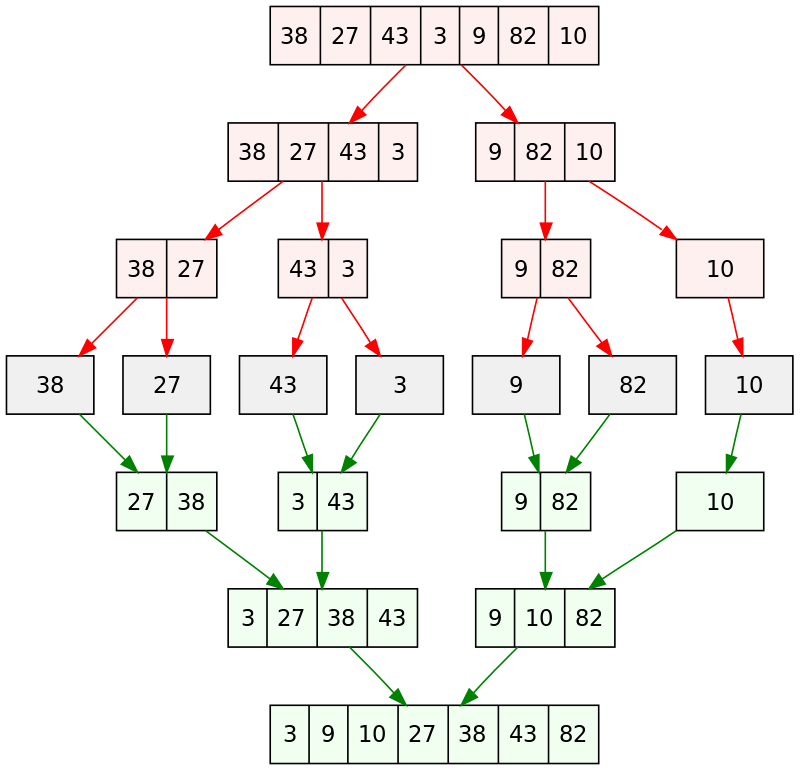
\includegraphics[height=0.7\paperheight]{imagens/mergesort.png}\\
	\tiny{Fonte: \url{https://en.wikipedia.org/wiki/Merge_sort}}
\end{figure}
\end{column}
\begin{column}{0.4\linewidth}
\vspace{3mm}
\begin{itemize}
	\item A execução do algoritmo pode ser vista como uma árvore binária
	\item Cada nodo representa uma chamada recursiva do algoritmo \emph{Merge Sort}
	\item Nodos recebem sequências de entrada para serem processadas e, por fim, geram sequências de saída ordenadas
\end{itemize}
\end{column}
\end{columns}
\end{frame}

%-------------------------------------------------------
\begin{frame}\frametitle{\emph{Merge Sort}: Implementação}
\lstinputlisting[basicstyle=\ttfamily\scriptsize]{src/mergeSort.cpp}
\end{frame}

%-------------------------------------------------------
\begin{frame}\frametitle{\emph{Merge Sort}: Desempenho [*]}
\begin{columns}[T]
\begin{column}{0.4\linewidth}
\vspace{3mm}
\begin{itemize}
	\item O tamanho da sequência de entrada é a metade a cada chamada recursiva
	\item A árvore associada a uma execução do algoritmo com uma sequência de tamanho $n$, tem altura $\log n$
	\item Conclusões:
	\begin{itemize}
		\item Altura da árvore é $\log n$
		\item Tempo gasto em cada nível: $O(n)$
		\item Tempo de execução: $O(n\log n)$
	\end{itemize}
\end{itemize}
\end{column}
\begin{column}{0.6\linewidth}
\vspace{-3mm}
\begin{figure}[h]
	\centering
	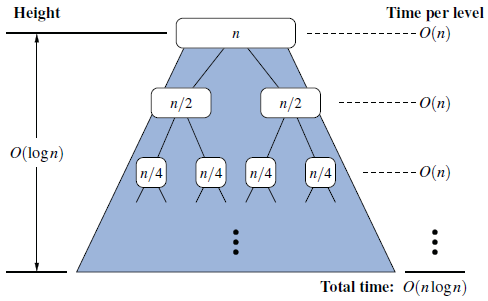
\includegraphics[height=0.6\paperheight]{imagens/mergesort_desempenho.png}
\end{figure}
\end{column}
\end{columns}
\end{frame}

%-------------------------------------------------------
\begin{frame}[fragile]\frametitle{\emph{Merge Sort}: Mais informações [*]}
\begin{itemize}
	\item \url{http://www.sorting-algorithms.com/merge-sort}
	\item \url{https://www.hackerearth.com/practice/algorithms/sorting/merge-sort/tutorial/}
\end{itemize}
\end{frame}

%=======================================================
\section{\emph{Quick Sort}}

%-------------------------------------------------------
\begin{frame}\frametitle{\emph{Quick Sort}}
\begin{itemize}
	\item Foi criado pelo cientista britânico Charles Antony Richard Hoare em 1959 e publicado em 1961
	\item É um algoritmo de ordenação por comparação que também utiliza o padrão ``Divisão e Conquista''
	\item Diferentemente do \emph{Merge Sort}, o \emph{Quick Sort} procura realizar a parte mais significativa do processamento \textbf{antes} das chamadas recursivas
	\item A estratégia geral subdivide-se nos seguintes passos:
	\begin{itemize}
		\item Escolhe-se um elemento da lista, denominado \textbf{pivô}
		\item Particionamento: a lista é reorganizada de forma que todos os elementos da lista menores que o pivô fiquem  à esquerda do pivô e que todos os elemenos maiores do que o pivô fiquem à sua direita -- o pivô estará em sua posição correta, porém  ``cercado'' por duas listas não ordenadas
		\item Essas duas listas são recursivamente ordenadas usando a mesma estratégia
	\end{itemize}
	\item Há variantes relacionadas principalmente à escolha do pivô, que o influencia o desempenho
\end{itemize}
\end{frame}

%-------------------------------------------------------
\begin{frame}[fragile]\frametitle{\emph{Quick Sort}: Escolha do Pivô}
\begin{itemize}
	\item A escolha do pivô influencia o desempenho
	\item Métodos:
	\begin{itemize}
		\item Hoare: escolhe o elemento central da coleção como pivô
		\item Lomuto: criado por Nico Lomuto, tipicamente escolhe o primeiro ou último elemento da coleção
		\item Pivô aleatório
		\item Valor intermediário entre primeiro, central e último elementos
	\end{itemize}
\end{itemize}
\end{frame}

%-------------------------------------------------------
\begin{frame}[fragile]\frametitle{\emph{Quick Sort}: Algoritmo (Hoare) \tiny{[Fonte: \url{https://pt.wikipedia.org/wiki/Quicksort}]}}
\fontsize{1}{6.5}\selectfont{
\begin{verbatim}
procedimento QuickSort(X[], IniVet, FimVet)
var
   i, j, pivo, aux
início
   i <- IniVet
   j <- FimVet
   pivo <- X[(IniVet + FimVet) div 2]
   enquanto(i <= j)
    |      enquanto (X[i] < pivo) faça
    |       |   i <- i + 1
    |      fimEnquanto
    |      enquanto (X[j] > pivo) faça
    |       |   j <- j - 1
    |      fimEnquanto
    |      se (i <= j) então
    |       |   aux  <- X[i]
    |       |   X[i] <- X[j]
    |       |   X[j] <- aux
    |       |   i <- i + 1
    |       |   j <- j - 1
    |      fimSe
   fimEnquanto
   se (IniVet < j) então
    |  QuickSort(X, IniVet, j)
   fimSe
   se (i < FimVet) então
    |  QuickSort(X, i, FimVet)
   fimSe
fimProcedimento
\end{verbatim}
}
\end{frame}

%-------------------------------------------------------
\begin{frame}[fragile]\frametitle{\emph{Quick Sort}: Algoritmo (Lomuto) \tiny{[Fonte: \url{https://pt.wikipedia.org/wiki/Quicksort}]}}
%\fontsize{1}{6.5}\selectfont{
\scriptsize{
\begin{verbatim}
algorithm quicksort(A, lo, hi) is
    if lo < hi then
        p := particiona(A, lo, hi)
        quicksort(A, lo, p – 1)
        quicksort(A, p + 1, hi)

algorithm particiona(A, lo, hi) is
    pivot := A[hi]
    i := lo - 1    
    for j := lo to hi - 1 do
        if A[j] < pivot then
            i := i + 1
            swap A[i] with A[j]
    if pivot < A[i + 1] then
        swap A[i + 1] with A[hi]
    return i + 1
\end{verbatim}
}
\end{frame}

%-------------------------------------------------------
\begin{frame}[fragile]\frametitle{\emph{Quick Sort}: Análise}
\begin{itemize}
	\item Se a \textbf{posição do pivô} escolhido for \textbf{central}, o \emph{Quick Sort} consegue duas subcoleções de tamanhos próximos
	\begin{itemize}
		\item Se isso \textbf{sempre} ocorresse, a altura da árvore de execução seria $O(\log{n})$
		\item Como em cada nível o tempo de execução será $O(n)$
		\item Então, o \textbf{melhor} tempo de execução do algoritmo poderia ser definido como $O(n\log{n})$
	\end{itemize}
	\item Por outro lado, no caso da variante Lomuto, que escolhe o último elemento como pivô, se a coleção já estiver ordenada, tem-se uma situação de pior caso, ou seja, $O(n^2)$
	\item Portanto, o desempenho do \emph{Quick Sort} está fortemente atrelado à escolha do pivô e à configuração ou posição inicial dos elementos na coleção
\end{itemize}
\end{frame}

%-------------------------------------------------------
\begin{frame}[fragile]\frametitle{\emph{Quick Sort}: Mais informações [*]}
\begin{itemize}
	\item \url{https://en.wikipedia.org/wiki/Quicksort}
	\item \url{http://www.sorting-algorithms.com/quick-sort}
	\item \url{https://www.hackerearth.com/practice/algorithms/sorting/quick-sort/tutorial/}
\end{itemize}
\end{frame}

%=======================================================
\section{Comparação}

%-------------------------------------------------------
\begin{frame}[fragile]\frametitle{Comparação}
\begin{itemize}
	\item Definir qual é o ``melhor'' algoritmo de ordenação nem sempre é fácil
	\item Há muitas variações, tanto nas implementações dos algoritmos quanto nas configurações de coleções (ordendada, invertida, aleatória, com muitos elementos duplicados, sem elementos duplicados, etc.)
	\item Até mesmo o \emph{Bubble Sort} pode apresentar o melhor desempenho para uma configuração específica
	\item Mas há alguns fatores que devem ser considerados...
\end{itemize}
\end{frame}

%-------------------------------------------------------
\begin{frame}[fragile]\frametitle{Estabilidade [*]}
\begin{itemize}	
	\item Um algoritmo de ordenação é estável (\emph{stable}) se não altera a posição relativa dos elementos que têm o mesmo valor
	\item Exemplo:
	\begin{itemize}
		\item Coleção inicial:
\begin{verbatim}
{ {"João", 21}, {"Ana", 55}, {"João", 13"}, {"Beto", 34}, {"Yuri", 23} }
\end{verbatim}
		\item Coleção ordenada por um algoritmo estável:
\begin{verbatim}
{ {"Ana", 55}, {"Beto", 34}, {"João", 21}, {"João", 13"}, {"Yuri", 23} }
\end{verbatim}
		\item Coleção ordenada por um algoritmo instável:
\begin{verbatim}
{ {"Ana", 55}, {"Beto", 34}, {"João", 13"}, {"João", 21}, {"Yuri", 23} }
\end{verbatim}
	\end{itemize}
\end{itemize}
\end{frame}

%-------------------------------------------------------
\begin{frame}\frametitle{Comparação dos Algoritmos quanto à Estabilidade}
\begin{itemize}	
	\item São estáveis:
	\begin{itemize}	
		\item \emph{Bubble Sort}
		\item \emph{Insertion Sort}
		\item \emph{Merge Sort}
	\end{itemize}
	\item São instáveis:
	\begin{itemize}	
		\item \emph{Selection Sort}
		\item \emph{Quick Sort}
	\end{itemize}
\end{itemize}
\end{frame}

%-------------------------------------------------------
\begin{frame}\frametitle{Armazenamento}
\begin{itemize}	
	\item Versões recursivas dos algoritmos necessitarão de memória da pilha
	\begin{itemize}	
		\item No \emph{Merge Sort} e \emph{Quick Sort}, o número máximo de chamadas recursivas aninhadas (ativas em determinado momento), em geral, será $O(\log{n})$
		\item Cuidado: implementações recursivas de outros algoritmos de ordenação podem gerar $O(n)$ chamadas recursivas aninhadas
	\end{itemize}
	\item Algoritmos de ordenação \emph{in-place} utilizam apenas o espaço da própria coleção para realizar a ordenação, NÃO necessitando de áreas de memória auxiliares
	\begin{itemize}	
		\item \emph{Merge Sort}, por exemplo, precisa de um vetor auxiliar
	\end{itemize}
	\end{itemize}
\end{frame}

%-------------------------------------------------------
\begin{frame}\frametitle{\emph{Bubble Sort}}
\begin{itemize}
	\item Complexidade: $O(n^2)$ (pior caso) ou $O(n)$ (melhor caso, considerando a implementação otimizada)
	\item É simples de ser implementado
	\item É estável
	\item Não necessita de um vetor auxiliar (\emph{in-place}), ocupando menos memória
	\item NÃO é recomendado para coleções grandes
\end{itemize}
\end{frame}

%-------------------------------------------------------
\begin{frame}\frametitle{\emph{Selection Sort}}
\begin{itemize}
	\item Complexidade: $O(n^2)$
	\item É simples de ser implementado
	\item Não necessita de um vetor auxiliar (\emph{in-place}), ocupando menos memória
	\item É relativamente rápido para pequenas coleções
	\item É um dos mais lentos para coleções grandes
	\item NÃO é estável
	\item Executa SEMPRE $(n^2-n)/2$ comparações
\end{itemize}
\end{frame}

%-------------------------------------------------------
\begin{frame}\frametitle{\emph{Insertion Sort}}
\begin{itemize}
	\item Complexidade: $O(n^2)$ (pior caso) ou $O(n)$ (melhor caso)
	\item É estável
	\item Não necessita de um vetor auxiliar (\emph{in-place}), ocupando menos memória
	\item Tem desempenho razoável principalmente para pequenas coleções (tamanho da ordem de dezenas)
	\item Eficiente para ordenação de coleções ``quase'' ordenadas
\end{itemize}
\end{frame}

%-------------------------------------------------------
\begin{frame}\frametitle{\emph{Merge Sort}}
\begin{itemize}
	\item Complexidade: $O(n\log{n})$ (pior caso)
	\item É estável
	\item Tem bom desempenho para coleções grandes
	\item Necessita de um vetor auxiliar
\end{itemize}
\end{frame}

%-------------------------------------------------------
\begin{frame}\frametitle{\emph{Quick Sort}}
\begin{itemize}
	\item Complexidade: $O(n\log{n})$ (melhor caso) ou $(n^2)$ (pior caso)
	\item Tem um desempenho excelente para vetores grandes
	\item NÃO é estável
	\item A escolha do pivô pode comprometer o desempenho
	\item Análises experimentais mostram que, se a sequência de entrada couber na memória principal, versões \emph{in-place} do \emph{Quick Sort} executam mais rápido que o \emph{Merge Sort} [*]
\end{itemize}
\end{frame}

%-------------------------------------------------------
\begin{frame}\frametitle{Comparativo com Medição de Tempo}
\begin{itemize}
	\item Vetor de 10.000 inteiros em 3 configurações: ordenado, invertido e aleatório
	\item Tempos medidos em $\mu$s (microssegundos)
\begin{center}
\begin{tabular}{|c|c|c|c|}
\hline
\textbf{Algoritmo} & \textbf{Ordenado} & \textbf{Invertido} & \textbf{Aleatório}\\
\hline
\emph{Bubble Sort} & 117 & 192173 & 224400 \\
\hline
\emph{Selection Sort} & 135131 & 105908 & 106956\\
\hline
\emph{Insertion Sort} & 174 & 148203 & 58291\\
\hline
\emph{Merge Sort} & 4277 & 3879 & 6470\\
\hline
\emph{Quick Sort} (Hoare) & 1186 & 406 & 1587\\
\hline
\emph{Quick Sort} (Lomuto) & 203035 & 136896 & 1108\\
\hline
\end{tabular}
\end{center}
\end{itemize}
\end{frame}

%=======================================================
\section{Exercícios e Testes}

%-------------------------------------------------------
\begin{frame}\frametitle{Exercício 1}
\begin{enumerate}
	\item Implemente os algoritmos das duas versões de \emph{Quick Sort} apresentadas nestas lâminas em C/C++ e teste as suas implementações com o código da página a seguir.
\end{enumerate}
\end{frame}

%-------------------------------------------------------
\begin{frame}\frametitle{Exercício 1}
\fontsize{1}{5}\selectfont{
\lstinputlisting{src/quickSortMain.cpp}
}
\end{frame}

%-------------------------------------------------------
\begin{frame}\frametitle{Exercícios 2, 3 e 4}
\begin{enumerate}
        \setcounter{enumi}{1}
	\item Adapte o código com a função \texttt{main()}, da lâmina anterior, para rodá-lo com as implementações de \emph{Bubble Sort}, \emph{Selection Sort}, \emph{Insertion Sort} e \emph{Merge Sort} (apresentadas nestas lâminas). Compare os tempos de execução de todas as implementações de algoritmos de ordenação.
	\item O código da função \texttt{main()}, da lâmina anterior, executa testes com um vetor já ordenado (em ordem crescente), com um vetor invertido (ordenado em ordem decrescente) e com um vetor com valores aleatórios. Crie uma nova configuração de teste para um vetor com alto número de elementos duplicados, e teste todos os algoritmos para esta nova configuração.
	\item Procure outros algoritmos de ordenação na Internet, implemente-os e adapte essas implementações para funcionarem no mesmo padrão dos testes executados anteriormente.
\end{enumerate}
\end{frame}

%=======================================================
\section{Créditos}

%-------------------------------------------------------
\begin{frame}\frametitle{Créditos}
\begin{itemize}
	\item Estas lâminas contêm trechos adaptados de materiais criados e disponibilizados pela professora Isabel Harb Manssour [*].
\end{itemize}
\end{frame}

%=======================================================
\section{Soluções}

%-------------------------------------------------------
\begin{frame}\frametitle{Solução: \emph{Quick Sort} (Hoare) em C/C++}
\lstinputlisting[basicstyle=\ttfamily\scriptsize]{src/quickSort1.cpp}
\end{frame}

%-------------------------------------------------------
\begin{frame}\frametitle{Solução: \emph{Quick Sort} (Lomuto) em C/C++}
\lstinputlisting[basicstyle=\ttfamily\tiny]{src/quickSort2.cpp}
\end{frame}

%-------------------------------------------------------
\end{document}

